\documentclass[12pt]{amsart}
\usepackage[T1]{fontenc}
\usepackage[utf8]{inputenc}

\usepackage[top=1.95cm, bottom=1.95cm, left=2.35cm, right=2.35cm]{geometry}

\usepackage{amsmath}
\usepackage{amssymb}
\usepackage{enumitem}
\usepackage{multicol}
\usepackage[french]{babel}
\usepackage[
    type={CC},
    modifier={by-nc-sa},
	version={4.0},
]{doclicense}

\usepackage{lymath}

\DeclareMathOperator{\taille}{\tau}

\newtheorem{fact}{Fait}
\newtheorem*{proof*}{Preuve}

\setlength\parindent{0pt}


\newcommand\squote[1]{\og #1 \fg{}}


\begin{document}

\title{BROUILLON - Faire des additions sur une parabole}
\author{Christophe BAL}
\date{17 Juillet 2019 - 27 Juillet 2019}
\maketitle


\vspace{-.9em}


\begin{center}
	\hrule\vspace{.3em}
	{
		\fontsize{1.35em}{1em}\selectfont
		\textbf{Mentions \og légales \fg}
	}
			
	\vspace{0.45em}
	\doclicenseThis
	\hrule
\end{center}



\setcounter{tocdepth}{2}
\tableofcontents



\section{\texorpdfstring{Comment additionner des nombres grâce à la parabole d'équation $y = x^2$}%
                        {Comment additionner des nombres grâce à la parabole d'équation y = x**2}}

Dans un repère orthogonal, donnons nous la parabole $\geoset{P} : y = x^2$ . Plaçons-y les points $A$ , $B$ et $S$ d'abscisses respectives $a$ , $b$ et  $s = a + b$ .
Observez
\footnote{
	Le lieu de téléchargement de ce document contient un fichier GeoGebra \texttt{base-tool.ggb} manipulable dynamiquement pour vérifier combien il est aisé de conjecturer quelque chose.
}
les trois cas ci-dessous et essayez de conjecturer quelque chose \emph{(la réponse est donnée dans la page suivante)}
\footnote{
	On peut géométriquement additionner modulo $2 \pi$ sur un cercle.
	Or $x^2 - y^2$ et $x^2 - y$ sont des formes quadratiques avec des propriétés géométriques communes.
	C'est là l'origine de la recherche proposée ici.
}.


\vspace{2.5em}

\begin{multicols}{2}
	\center
	\footnotesize
	\itshape
	
	\fbox{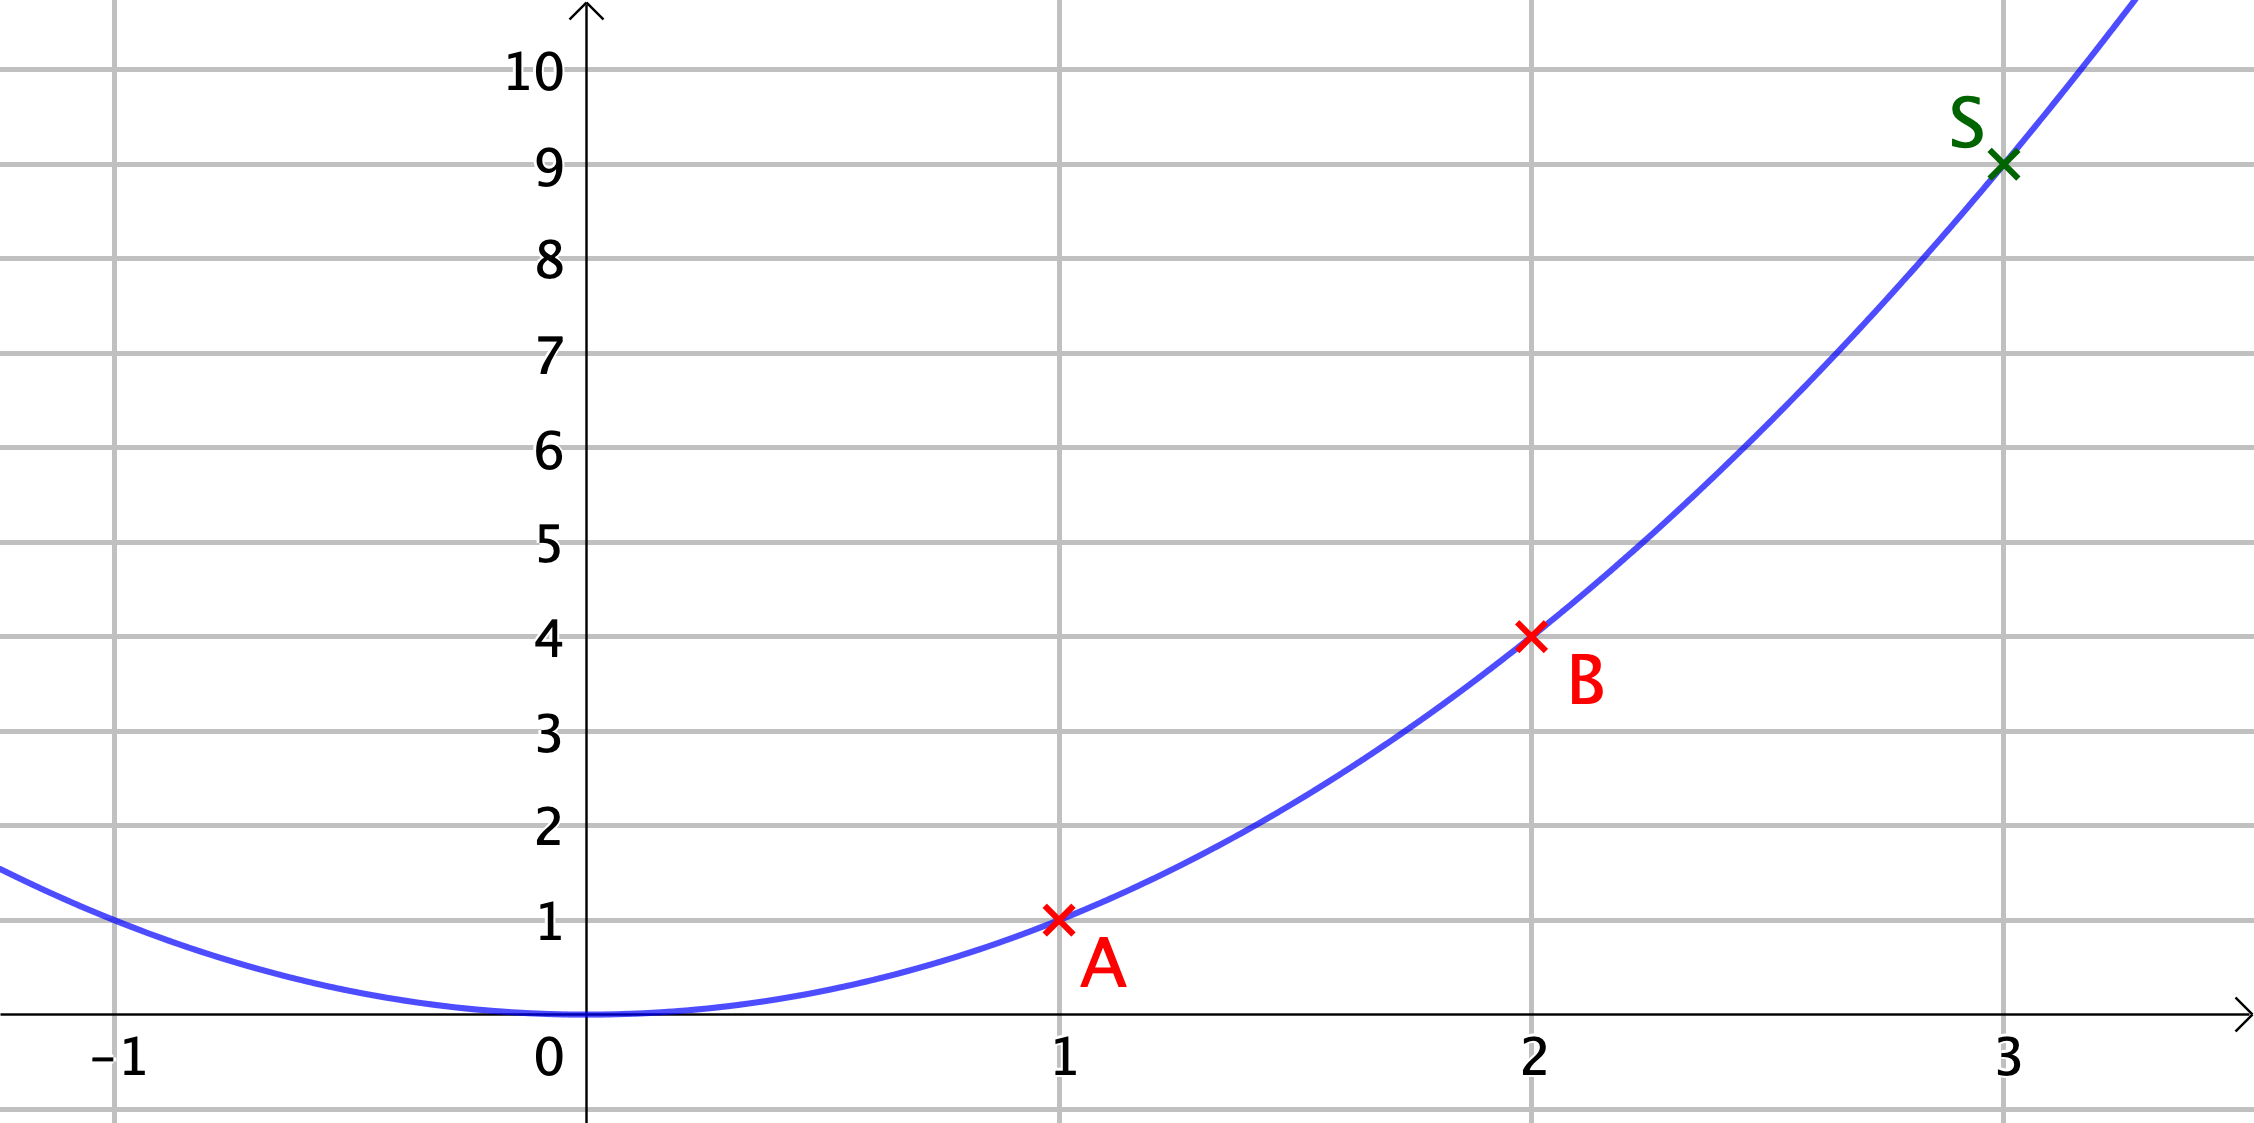
\includegraphics[scale = .8]{addition-on-parabolas/conjecture/a-and-b-positive.png}}
	
	\smallskip
	Cas où $a > 0$ et $b > 0$

	\columnbreak
	
	\fbox{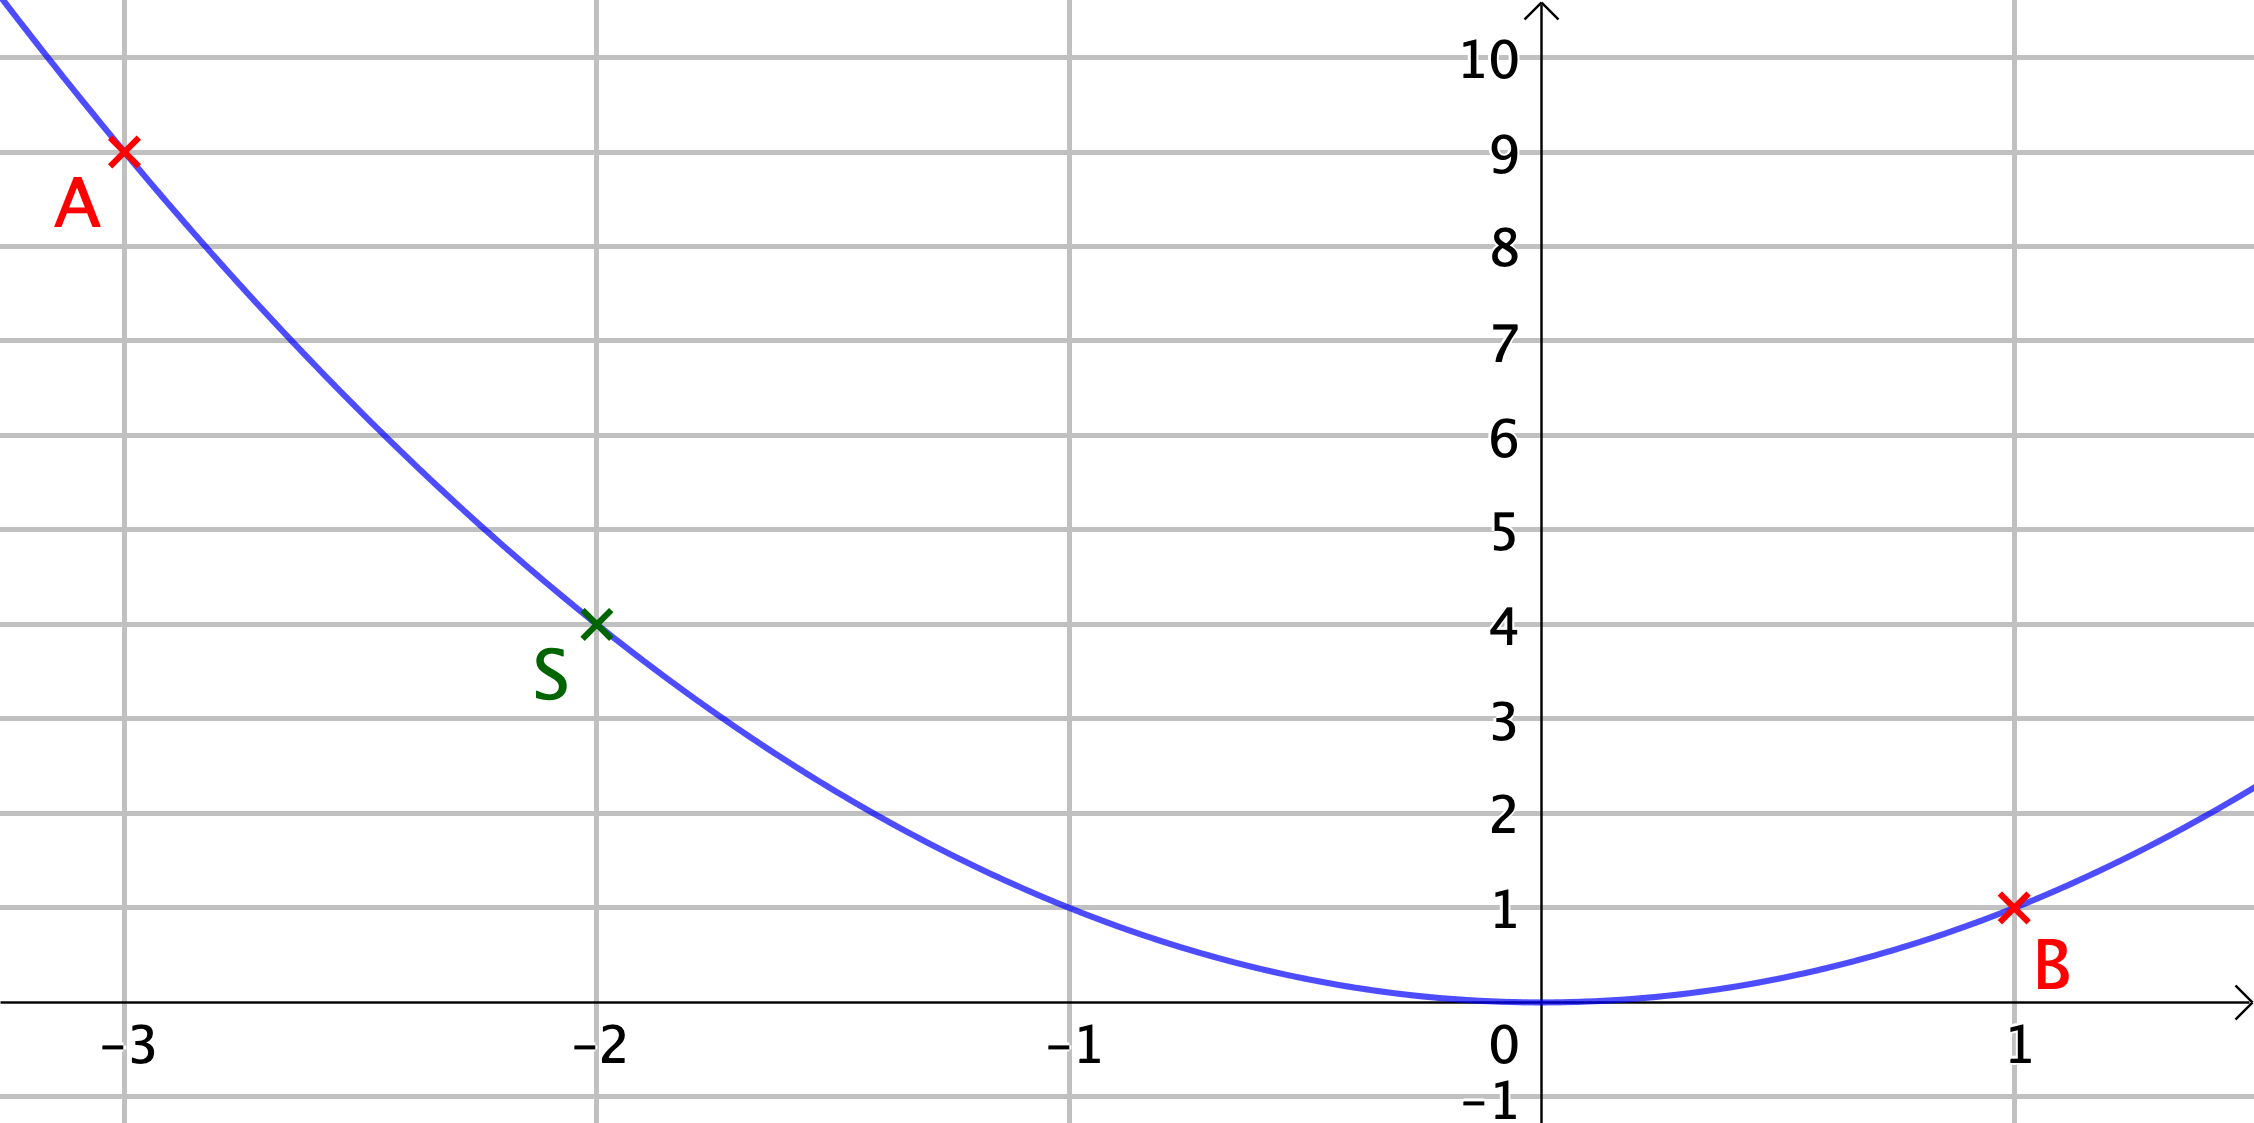
\includegraphics[scale = .8]{addition-on-parabolas/conjecture/a-and-b-diff-signs.png}}
	
	\smallskip
	Cas où $a < 0$ et $b > 0$
\end{multicols}
	
\begin{center}
	\footnotesize
	\itshape

	\fbox{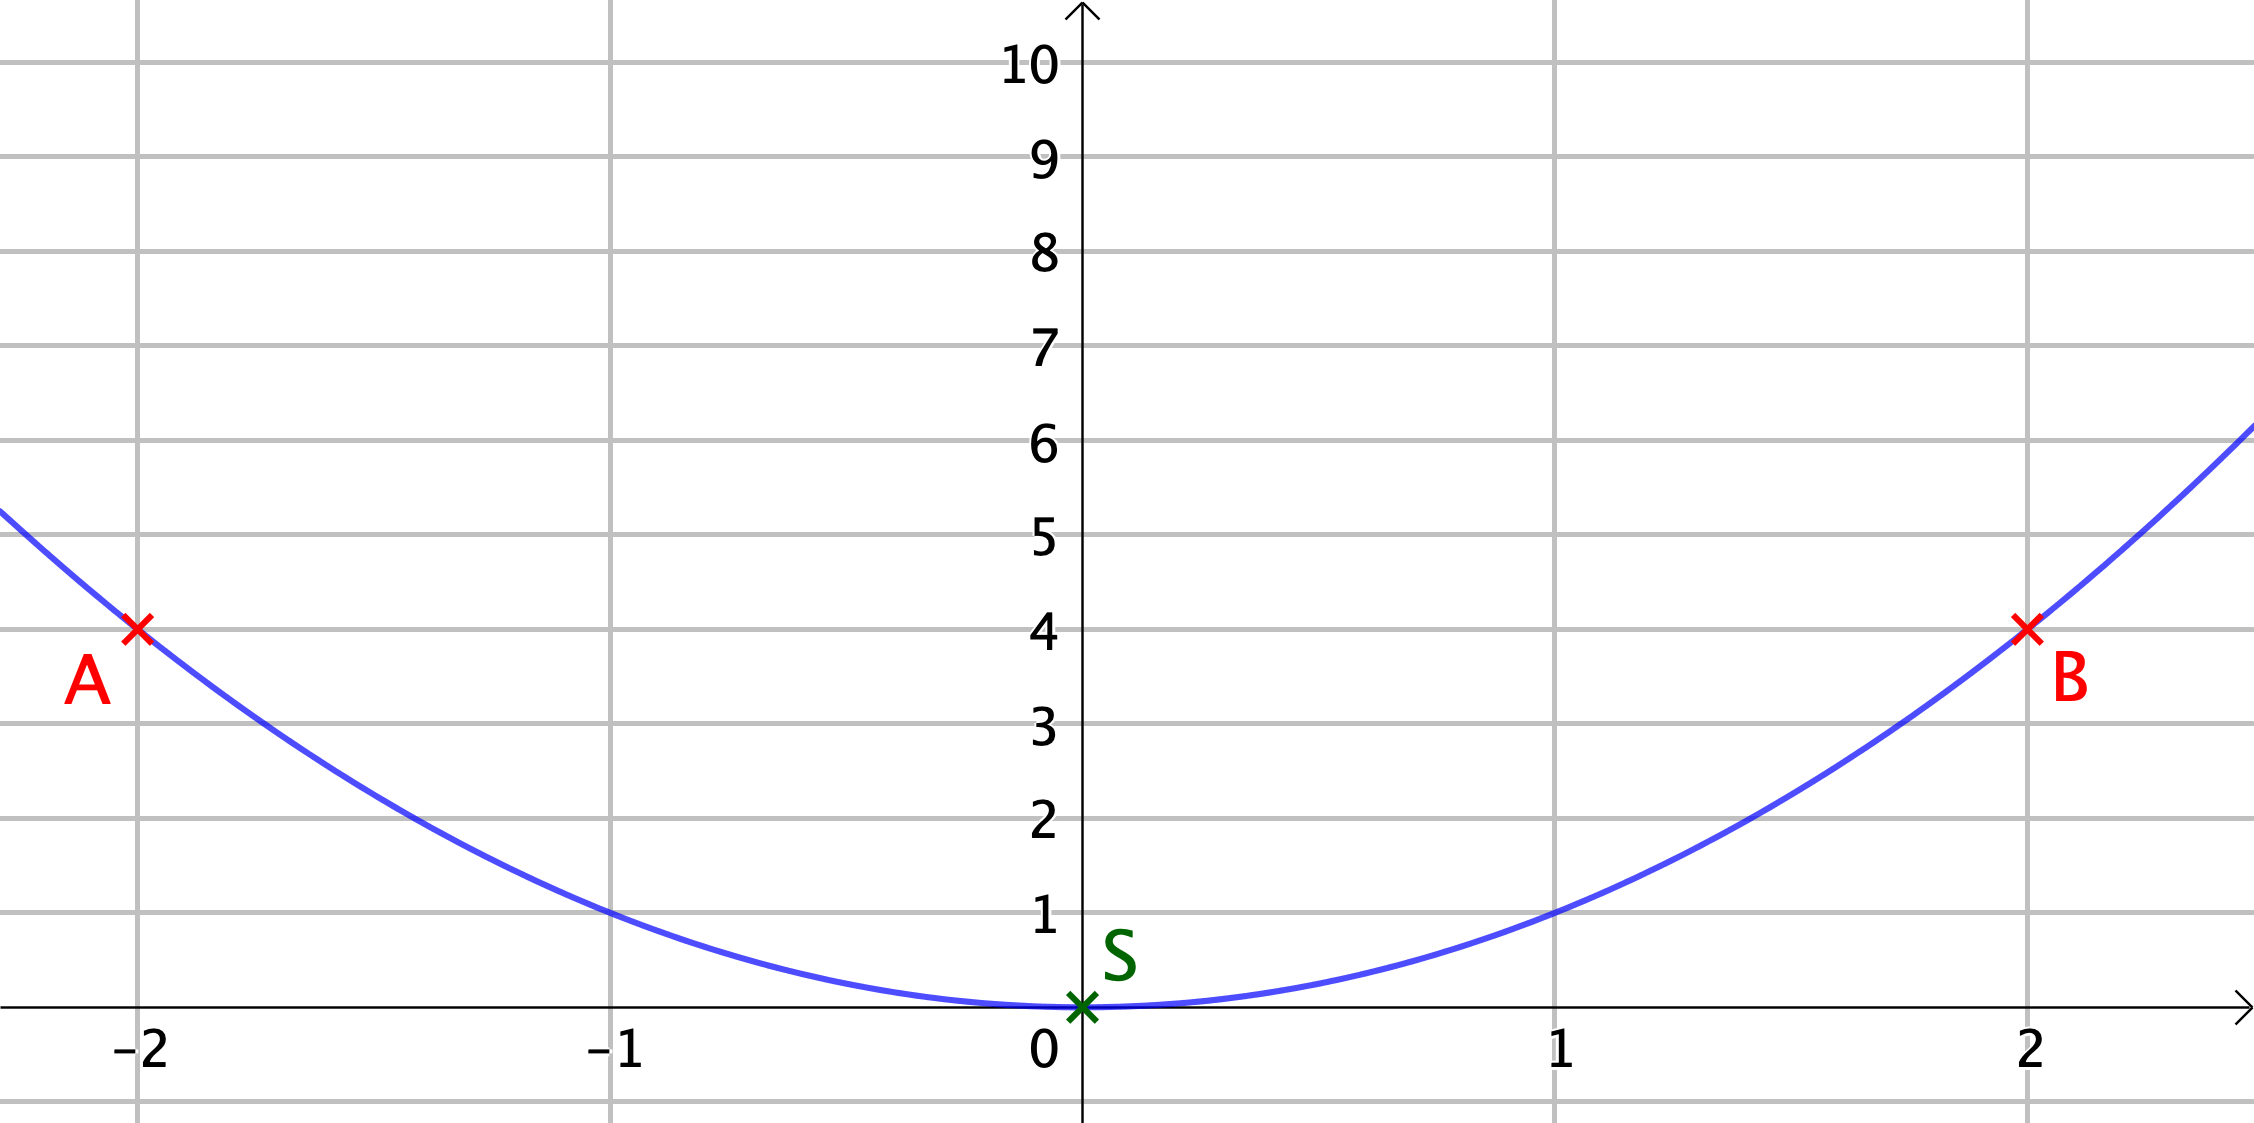
\includegraphics[scale = .8]{addition-on-parabolas/conjecture/a-and-b-opposite.png}}
	
	\smallskip
	Cas où $a = -b$
\end{center}


\newpage

Pour mieux voir ce qu'il se passe, traçons quelques droites. Voici ce que cela donne.

\begin{multicols}{2}
	\center
	\footnotesize
	\itshape

	\fbox{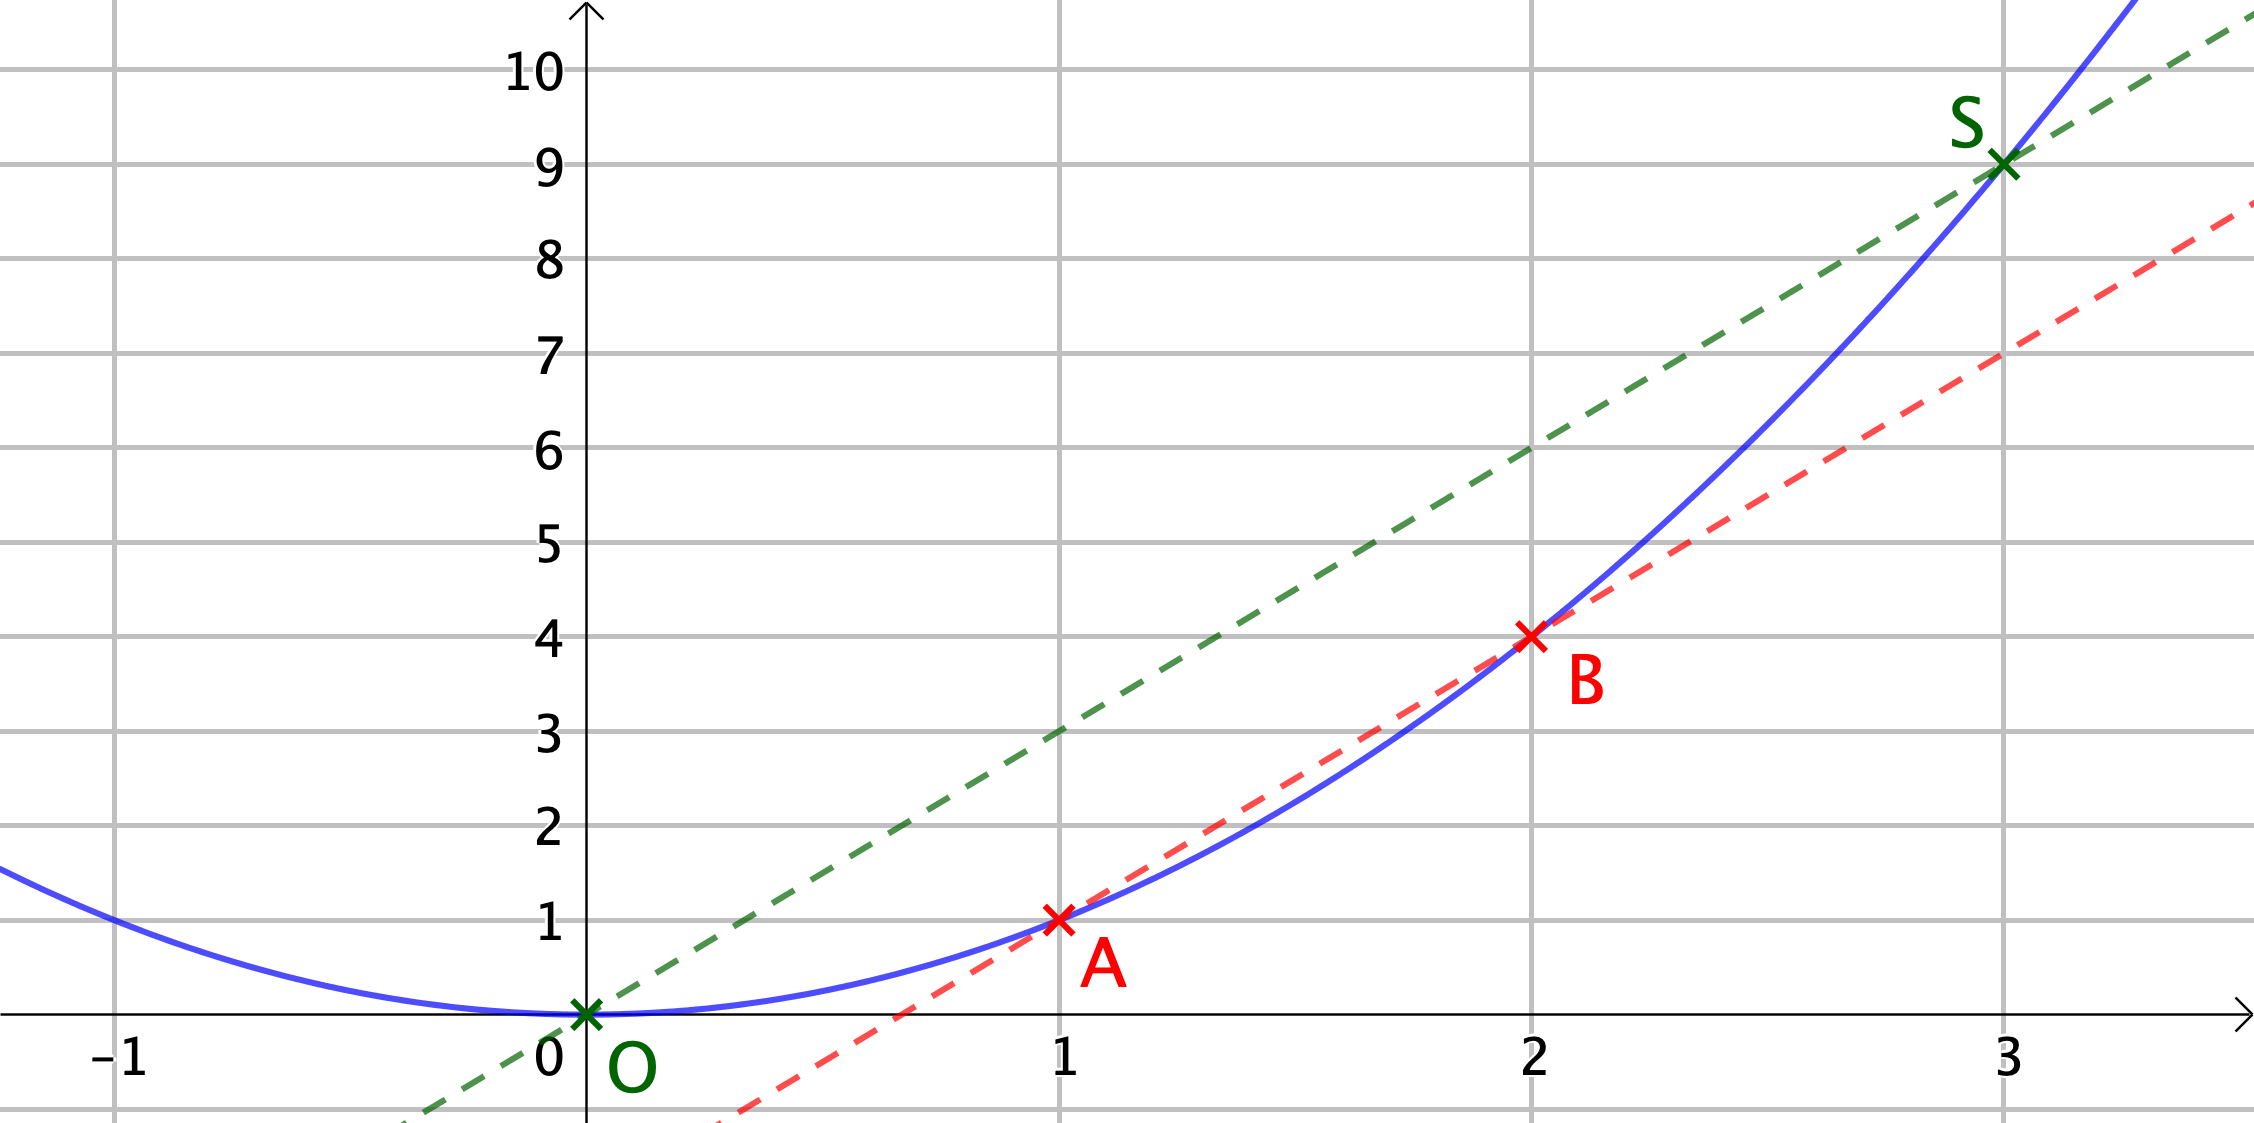
\includegraphics[scale = .8]{addition-on-parabolas/conjecture/a-and-b-positive-with-lines.png}}
	
	\smallskip
	Cas où $a > 0$ et $b > 0$

	\columnbreak
	
	\fbox{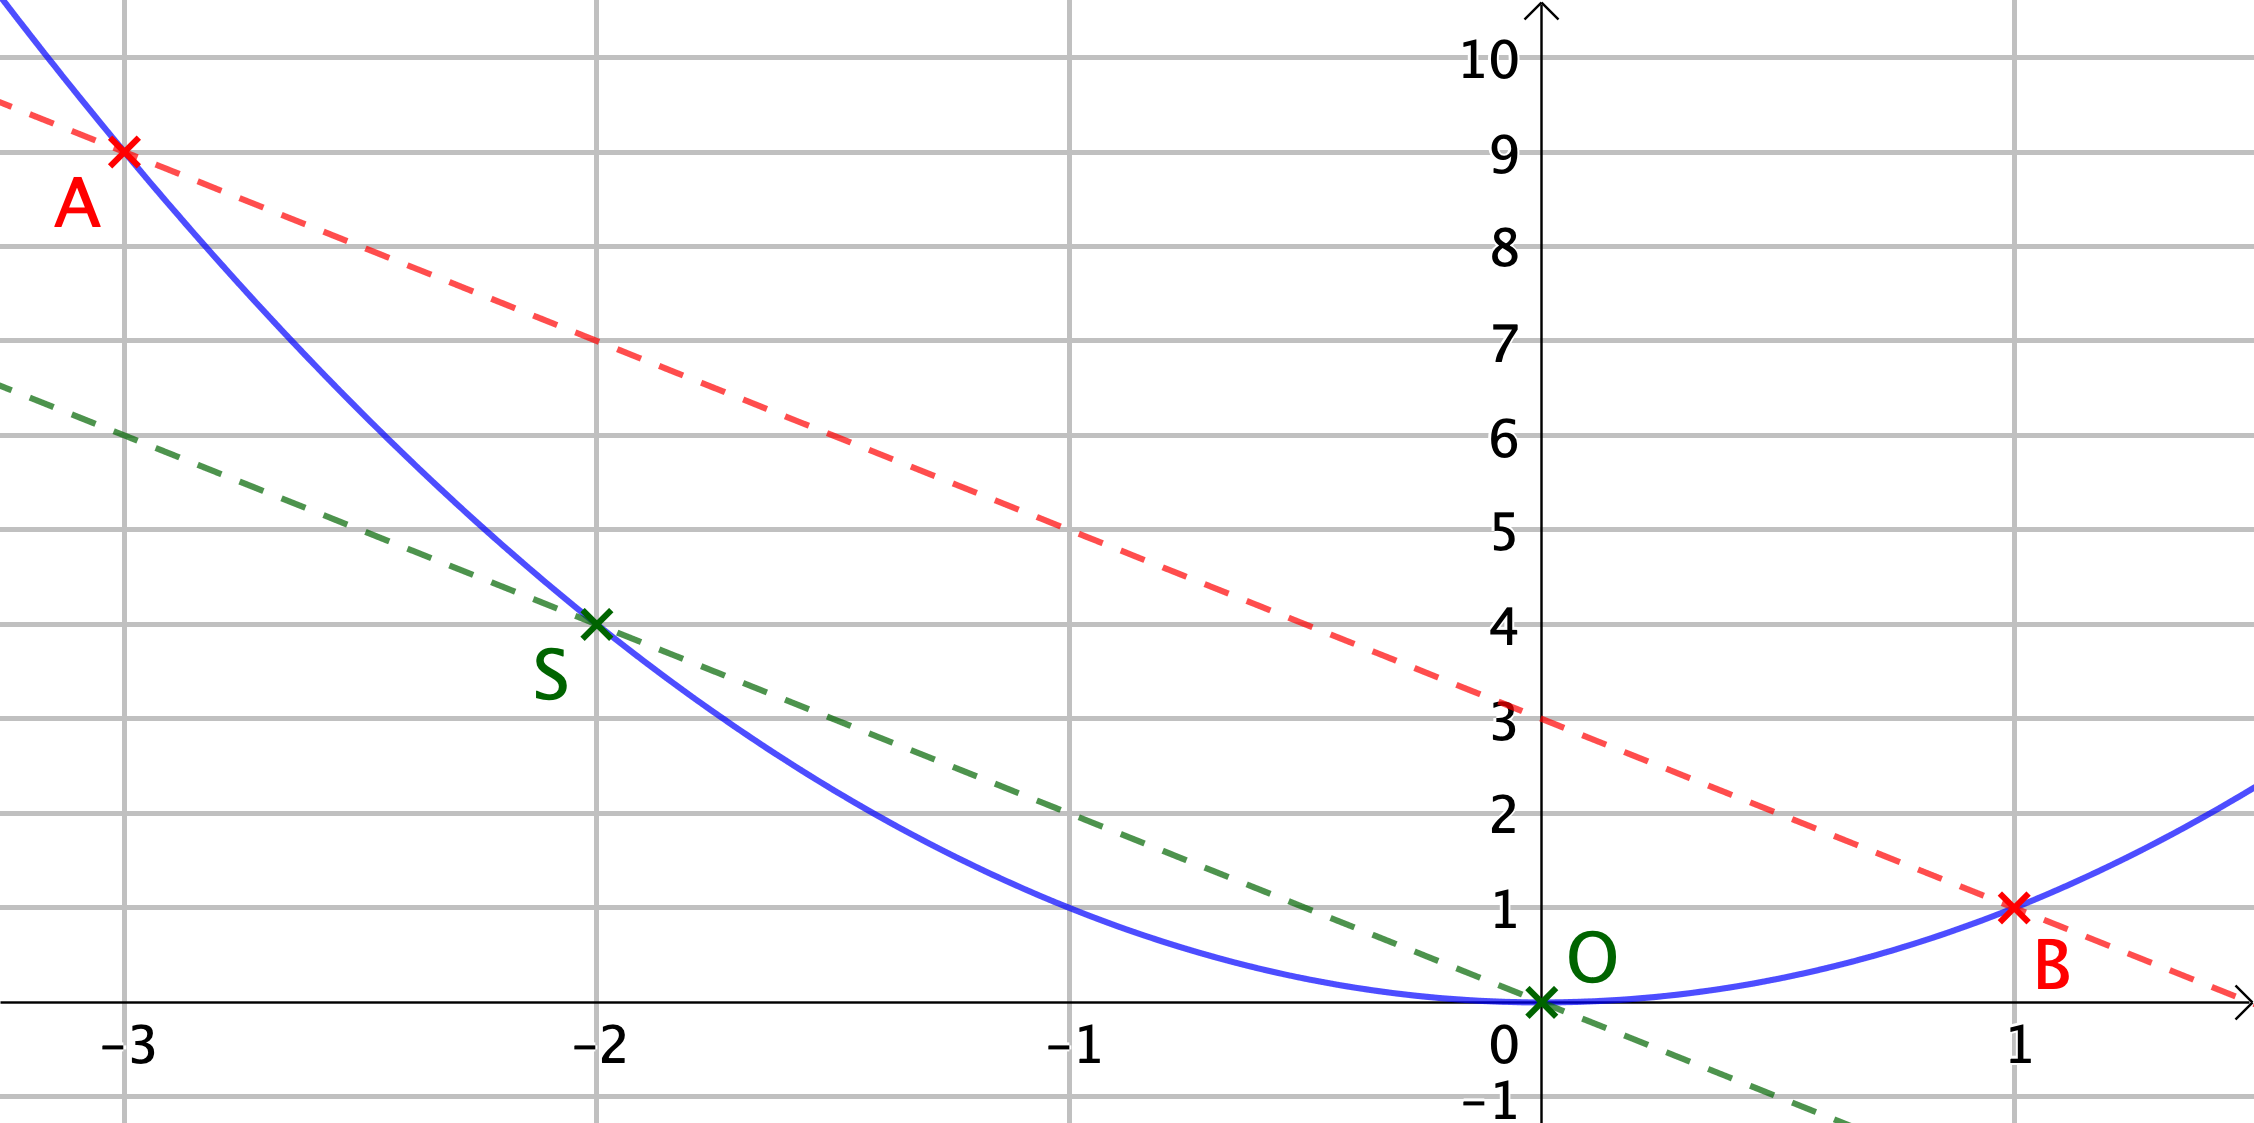
\includegraphics[scale = .8]{addition-on-parabolas/conjecture/a-and-b-diff-signs-with-lines.png}}
	
	\smallskip
	Cas où $a < 0$ et $b > 0$
\end{multicols}
	
\begin{center}
	\footnotesize
	\itshape

	\fbox{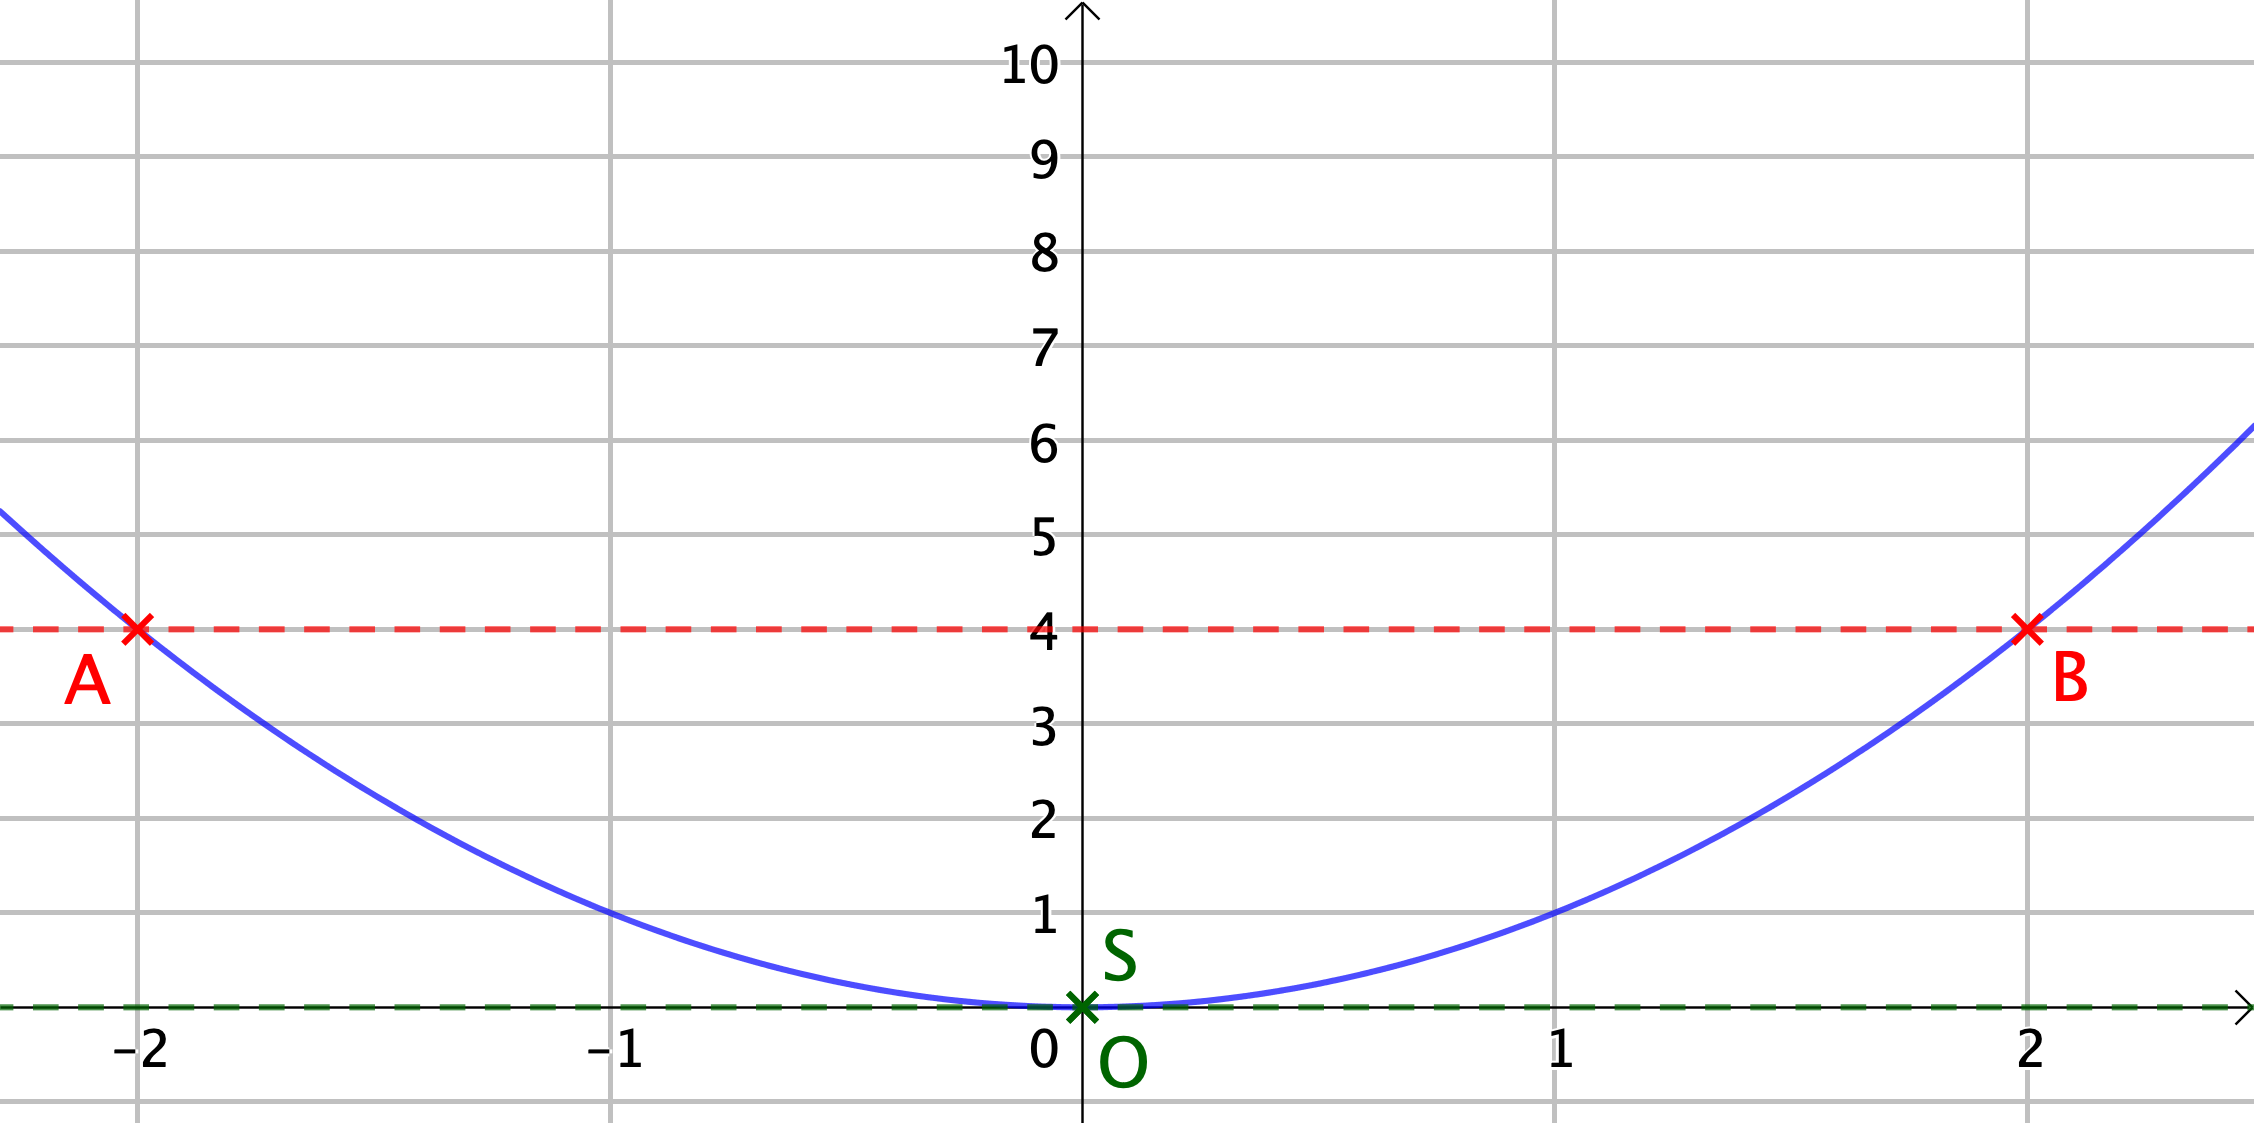
\includegraphics[scale = .8]{addition-on-parabolas/conjecture/a-and-b-opposite-with-lines.png}}
	
	\smallskip
	Cas où $a = -b$
\end{center}


\medskip

Il devient évident de conjecturer que le point $S$ se construit géométriquement comme suit.

\begin{enumerate}
	\item \label{point-1} Si $x_A \neq \pm \, x_B$ alors on construit la parallèle à $(AB)$ passant par $O$ l'origine du repère. Le point $S$ est le second point d'intersection de cette parallèle avec $\geoset{P}$  \emph{(notons qu'une droite coupe $\geoset{P}$ en au plus deux points)}.

	\item Si $x_A = - x_B$ alors $S = O$ . Notons au passage que l'on peut voir ceci comme un cas limite du précédent avec un point d'intersection \squote{double}.

	\item Si $x_A = x_B \neq 0$ , on procède comme au point (\ref{point-1}) mais avec la parallèle à la tangente en $A$ à la parabole $\geoset{P}$ .
\end{enumerate}


La section qui suit va valider cette conjecture qui donne un moyen très capillotracté de calculer une somme de deux réels via la parabole $\geoset{P}$ .
Plus sérieusement, la construction ci-dessus est une propriété géométrique très jolie de la parabole $\geoset{P}$ .




\section{Preuve de la validité de la conjecture} \label{proof}
\label{proof}

\textbf{Cas 1.} \emph{Supposons que $x_A \neq \pm \, x_B$ de sorte que $x_S \neq 0$ .}

\medskip

La droite $(AB)$ a pour pente
$\frac{y_A - y_B}{x_A - x_B} = \frac{a^2 - b^2}{a - b} = a + b$ .
De plus, la droite $(OS)$ qui passe par l'origine $O$ du repère a pour pente
$\frac{y_S}{x_S} = \frac{x_S^2}{x_S} = x_S = a + b$ .
Les droites $(AB)$ et $(OS)$ sont bien parallèles comme nous l'avons affirmé.


\bigskip

\textbf{Cas 2.} \emph{Supposons que $x_A = - x_B$ .}

\medskip

Comme $x_S = a + b = 0$ , nous avons bien $S = O$ .


\bigskip

\textbf{Cas 3.} \emph{Supposons que $x_A = x_B \neq 0$ .}

\medskip

Dans ce cas, $x_S = 2a \neq 0$ donc la droite $(OS)$ a pour pente
$x_S = 2a$ qui est bien la pente de la tangente en $A$ à la parabole $\geoset{P}$ .



\section{\texorpdfstring{Toute parabole d'équation $y = a x^2 + b x + c$ a une structure de groupe}%
                        {Toute parabole d'équation y = a x**2 + b x + c a une structure de groupe}}
      
Le procédé de construction que nous venons de prouver dans la section \ref{proof} se \emph{\og conserve \fg} par translations et dilatations verticales et horizontales.
Il se trouve que ce sont ces transformations qui permettent d'obtenir une parabole $\geoset{P}\,^\prime : y = a x^2 + b x + c$ , donc $a \neq 0$ , à partir de celle de la parabole $\geoset{P} : y = x^2$ .
Nous pouvons donc munir toute parabole $\geoset{P}\,^\prime : y = a x^2 + b x + c$ d'une structure de groupe isomorphe à celle de $(\RR ; +)$ , et ceci avec un procédé géométrique simple pour \emph{\og additionner \fg} sur $\geoset{P}\,^\prime$ . Que c'est joli !




\section{Une caractérisation analytique des fonctions trinomes nulles en zéro}
      
Finissons ce document avec un résultat plus technique en nous demandant quelles peuvent être les fonctions $f$ définies et dérivables sur $\RR$ qui vérifient les propriétés suivantes utilisées dans la démonstration de la section \ref{proof}.
\begin{enumerate}
	\item $\forall (a ; b) \in \RR^2$ , si $a \neq b$ alors $\frac{f(a) - f(b)}{a - b} = \frac{f(a + b)}{a + b}$ .

	\item $f$ est paire et $f(0) = 0$ .

	\item $\forall a \in \RRs$ , $f\,'(a) = \frac{f(2 a)}{2 a}$ . Notons que cette propriété est en fait une conséquence de la première via un passage à la limite de $b$ vers $a$ .
\end{enumerate}


\medskip


La fonction $f$ doit être une solution sur $\RR$ de l'équation différentielle $2 x \, y\,'(x) = y(2x)$ qui n'est pas très sympathique car d'un côté il a $x$ comme variable et de l'autre il y a $2x$ !
Pour avancer, nous allons nous restreindre au cas où $f$ est la restriction d'une fonction $\widetilde{f}$ définie et holomorphe sur $\CC$ , c'est à dire telle que $\forall \omega \in \CC$ , la limite $\displaystyle \lim_{\stackrel{\abs{z - \omega} \, \rightarrow \, 0}{z \neq \omega}} \frac{\widetilde{f}(z) - \widetilde{f}(\omega)}{z - \omega}$ existe dans $\CC$ .


On sait alors qu'il existe $R > 0$ tel que $\abs{z} < R$ implique
$\displaystyle \widetilde{f}(z) = \sum_{k = 0}^{+ \infty} c_k z^k$ , ce développement étant unique car $c_k = \frac{\derpow[k]{f}(0)}{k!}$ , et aussi que les éventuels zéros $\lambda$ de $\widetilde{f}$ sont isolés, c'est à dire qu'il existe un voisinage de $\lambda$ sur lequel $\widetilde{f}$ ne s'annule qu'en $\lambda$ . Nous admettrons ces deux faits de l'analyse complexe car les prouver nous amènerait trop loin.


\medskip

Nous admettrons aussi que $\forall x \in \RR$ , $2 x \, f\,'(x) = f(2x)$ implique $\forall z \in \CC$ , $2 z \, \widetilde{f}\,'(z) = \widetilde{f}(2z)$ \emph{(ceci vient principalement de la propriété des zéros isolés et du fait que toute fonction holomorphe l'est à tout ordre)}. 


\medskip

Dès que $\abs{z} < 0,5 R$ , nous avons alors :
\begin{flalign*}
	2 z \, \widetilde{f}\,'(z) = \widetilde{f}(2z)
		&\Longleftrightarrow
		2 z \sum_{k = 0}^{+ \infty} k c_k z^{k - 1}
		=
		\sum_{k = 0}^{+ \infty} c_k (2z)^k
		& \\
		&\Longleftrightarrow
		\sum_{k = 0}^{+ \infty} 2 k c_k z^k
		=
		\sum_{k = 0}^{+ \infty} c_k (2z)^k
		& \\
		&\Longleftrightarrow
		\forall k \in \NN \, , \, 2 k c_k = 2^k c_k
		& \\
		&\Longleftrightarrow
		c_1 
		\,\,
		\text{et}
		\,\,
		c_2
		\,\,
		\text{quelconques et}
		\,\,
		\forall k \in \NNs - \geneset{1 ; 2} \, , \, c_k = 0
		& \\
		&\Longleftrightarrow
		\widetilde{f}(z) = c_1 z + c_2 z^2
		& \\
\end{flalign*}

\vspace{-1em}


Le principe des zéros isolés et le fait que  $\widetilde{f}(z)$ et $c_1 z + c_2 z^2$ soient holomorphes sur $\CC$ nous donnent que $\widetilde{f}(z) = c_1 z + c_2 z^2$ sur $\CC$ tout entier, et donc $f(x) = c_1 x + c_2 x^2$ sur $\RR$ .


\medskip

Compte tenu de la section précédente, la condition nécessaire ci-dessus est aussi suffisante. Nous avons donc obtenu une caractérisation des fonctions trinômes nulles en zéro parmi les fonctions qui sont la restriction d'une fonction définie et holomorphe sur $\CC$ .


\end{document}
